\documentclass{standalone}

\usepackage{tikz}
\usetikzlibrary{calc}
\usetikzlibrary{patterns}

\newlength{\len}
\setlength{\len}{.5mm}

\begin{document}

\begin{tikzpicture}[x=\len, y=\len]

  \path (0, 0) node[anchor=south west]{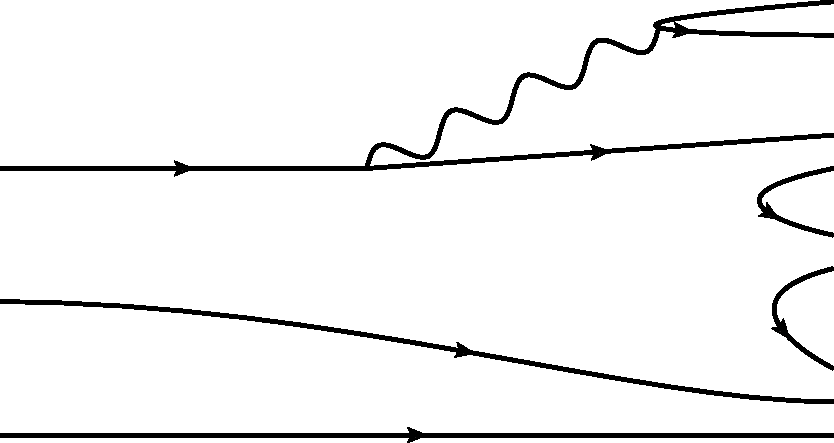
\includegraphics[width=100\len]{src/diagram-lb2dppipi-boldlines}};

  \path ( -7,  20) node{$\Lambda_b^0$};
  \path (  5,  40) node{$b$};
  \path (  5,  24) node{$d$};
  \path (  5,   6) node{$u$};

  \path ( 57,  50) node{$W^-$};
  \path ( 80,  42) node{$c$};
  \path ( 99,  32) node{$d$};
  \path (100,  16) node{$u$};

  \path (103,  55) node[anchor=west]{$\pi^-$};
  \path (103,  38) node[anchor=west]{$D^+$};
  \path (103,  26) node[anchor=west]{$\pi^-$};
  \path (103,   7) node[anchor=west]{$p$};

\end{tikzpicture}

\end{document}
